%chargedCorrBtoDPlots
%!TEX root = ../main.tex
%

%\section{$B^- \rightarrow D^0$ decays: additional plots}
\subsection{$B^- \rightarrow D^0$ decays: additional plots}
\label{chargedBtoD0App}

Figures \ref{fig:chargedBtoD_FOMvsR2_cut}-\ref{fig:chargedBtoD_FOMvsSigProb_cut} show the FOM values at various cuts 
on $foxWolframR2$ and SignalProbability variables respectively. After the cuts on the first two variables were optimized, the cut on $D^0_{CMS}$ is chosen 
considering the momenta distributions plotted on \ref{fig:chargedcorrD0_Pcms}: $p^{D^0 }_{CMS} > 1$ GeV/c$^2$ removes 
a good portion of background events while retaining most of the signal events.

\begin{figure}[H]
  %\centering
  {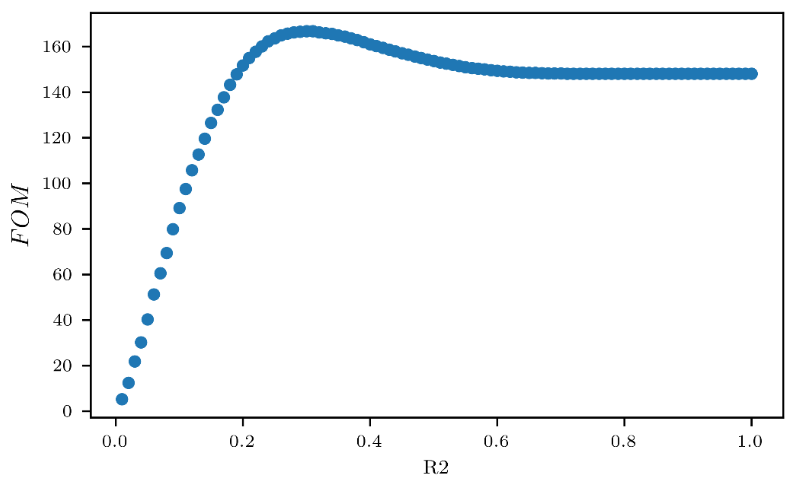
\includegraphics[width=0.75\textwidth]{A2-Appendix/figs/R2Optimisation_chargedB_D0Sample.png}}
  \caption{Figure of Merit values calculated at several cuts on the $foxWolframR2$ variable.}
  \label{fig:chargedBtoD_FOMvsR2_cut}
  \end{figure}
   


\begin{figure}[H]
    %\centering
    {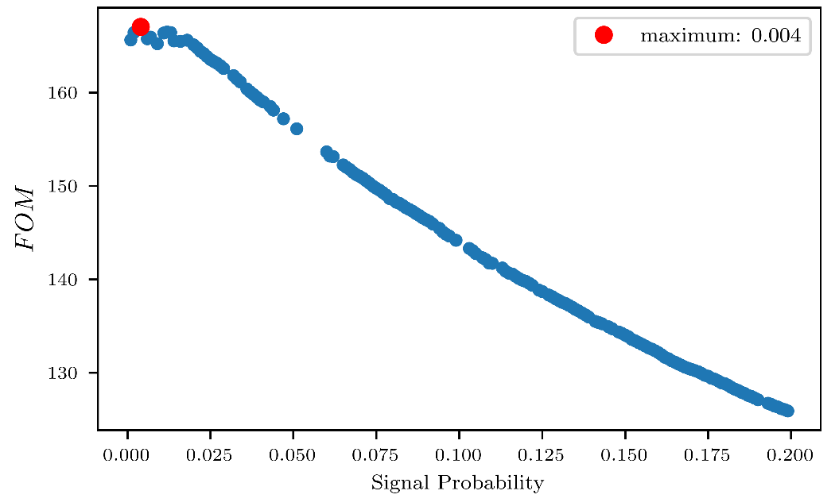
\includegraphics[width=0.75\textwidth]{A2-Appendix/figs/SigProbOptimisation_chargedB_D0Sample.png}}
    \caption{Figure of Merit values calculated at several cuts on the SignalProbability variable.}
    \label{fig:chargedBtoD_FOMvsSigProb_cut}
\end{figure}

\begin{figure}[H]
  %\centering
{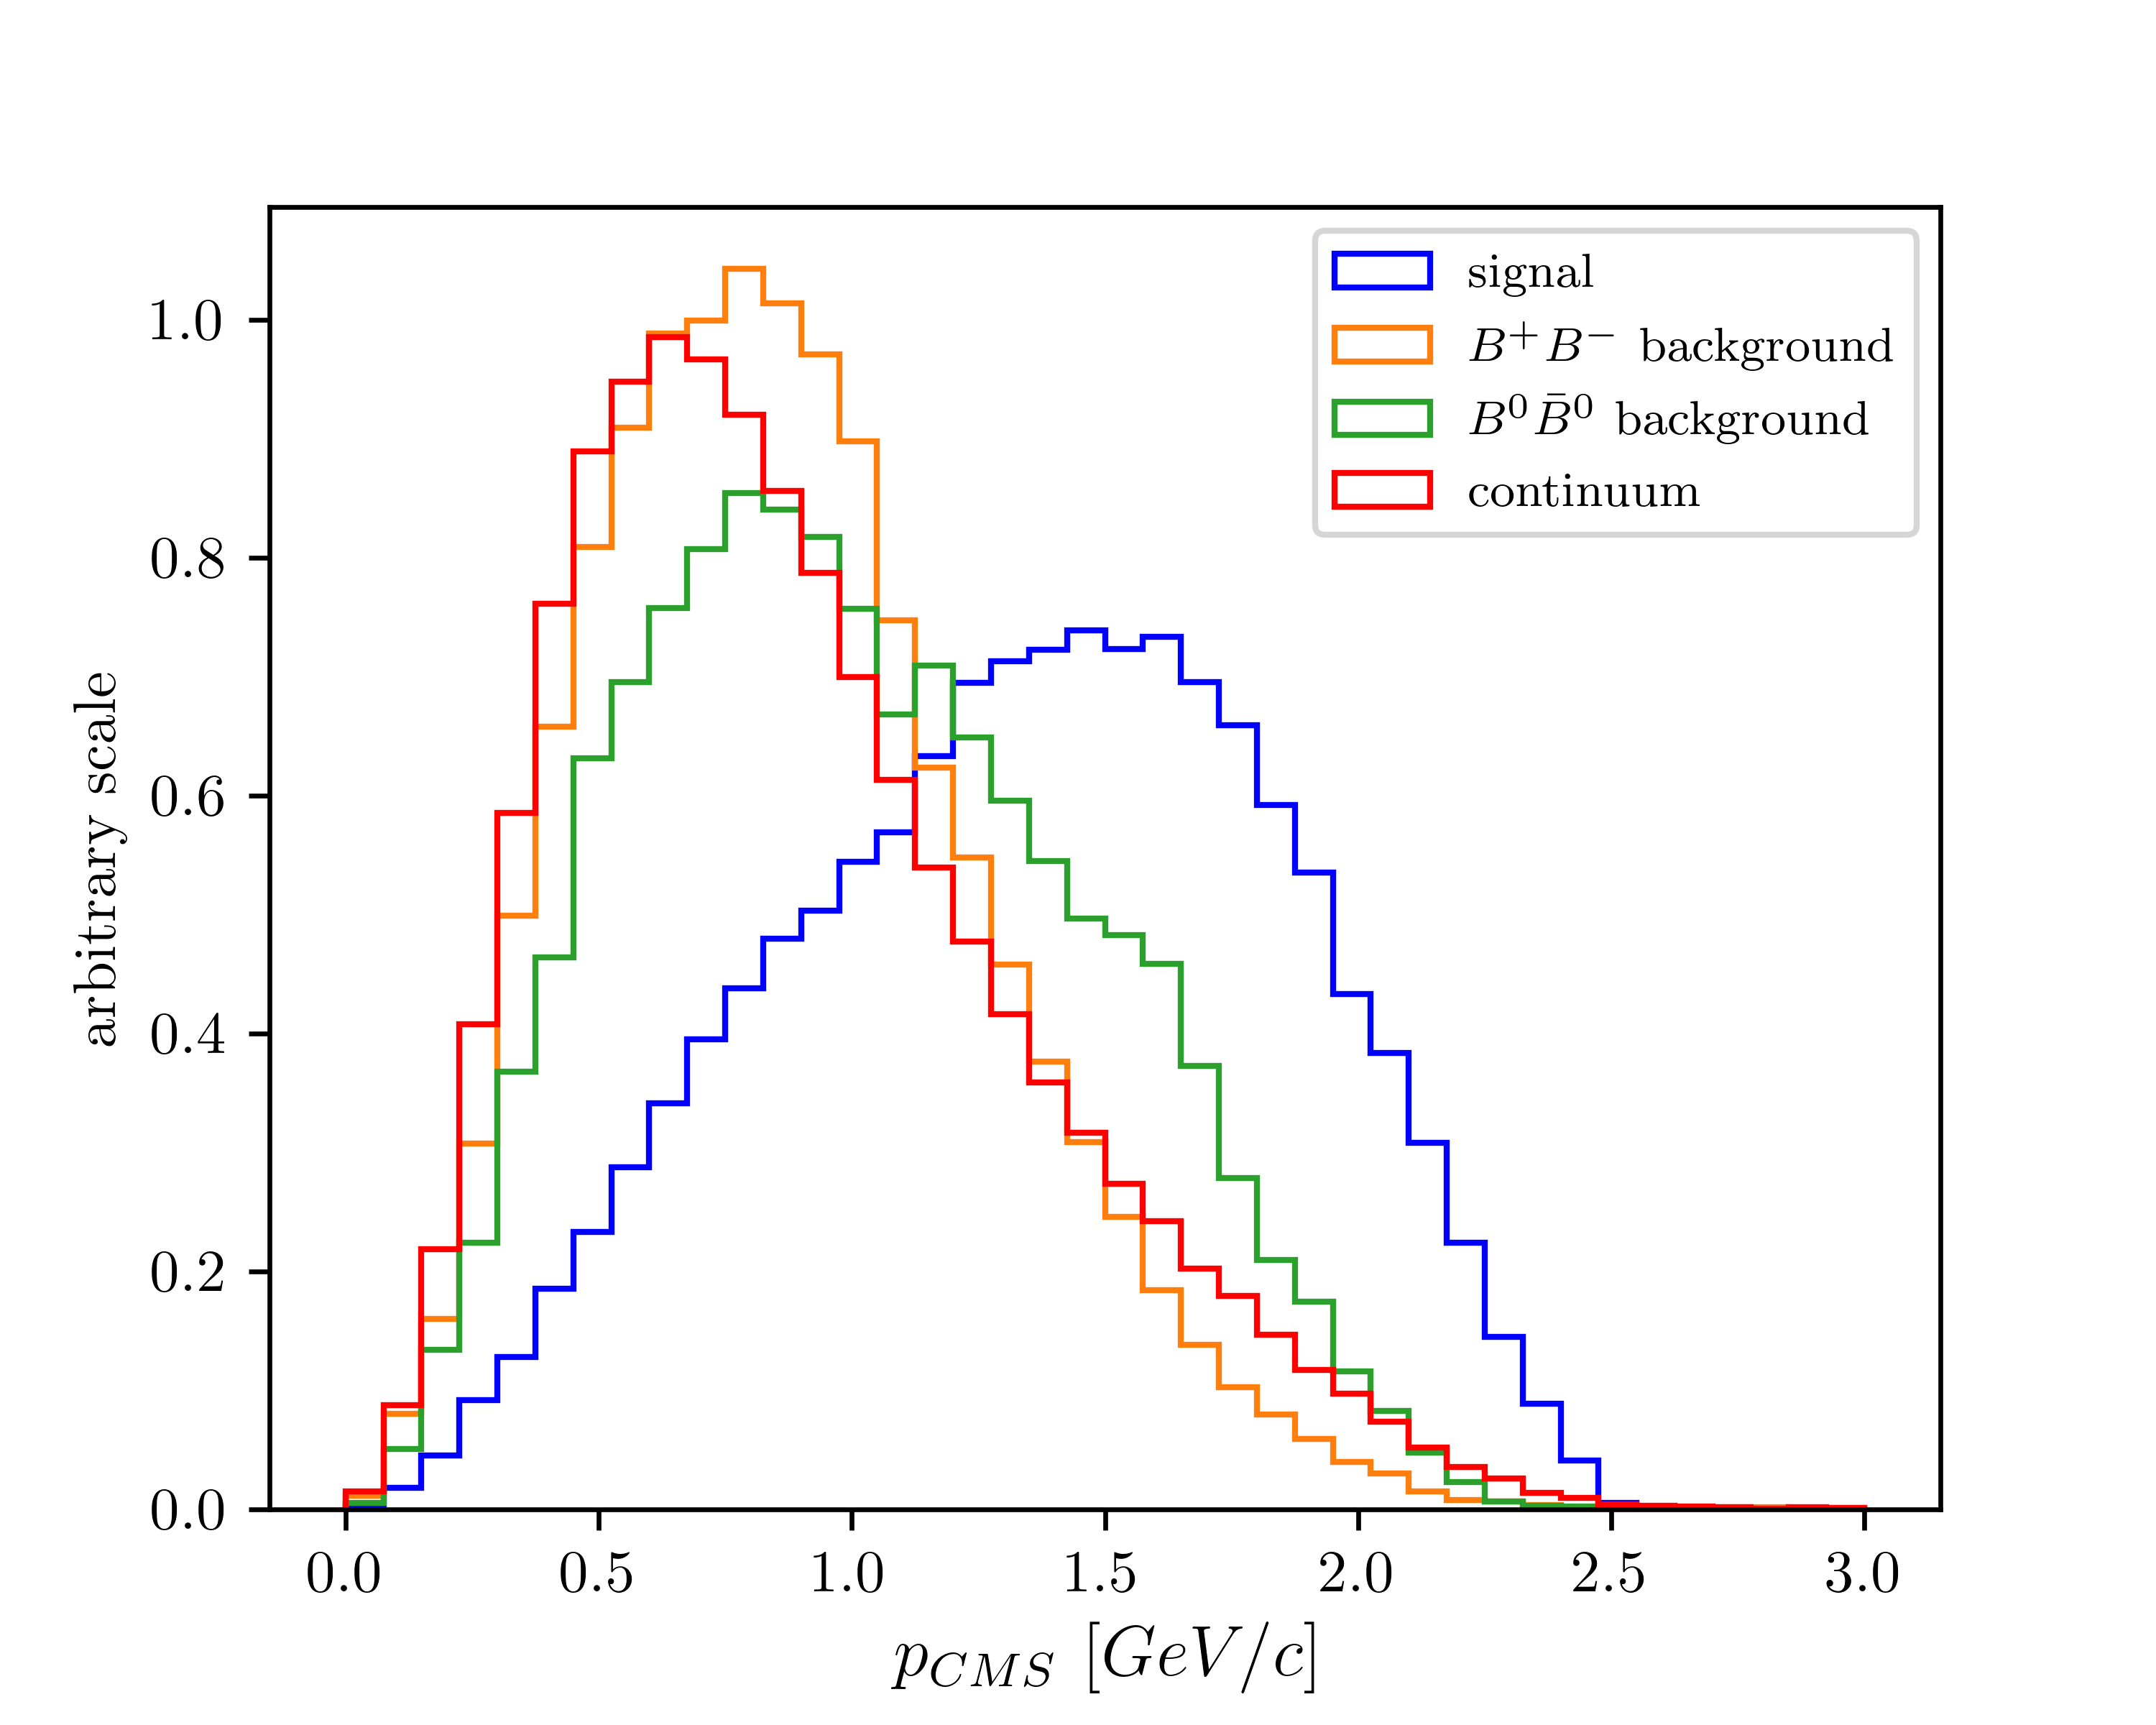
\includegraphics[width=0.75\textwidth]{A2-Appendix/figs/chargedBtoD0bar_Pcms_afterOpt.png}}
\caption{Distribution of  $D^0$ candidates momenta in the center of mass system after the cuts on $foxWolframR2$ 
and SignalProbability variables were applied.}
\label{fig:chargedcorrD0_Pcms}
\end{figure}
   

Figures \ref{fig:stream0Signal_window_chargedControlD0_Total_2DFit}-\ref{fig:InvM_Sideband_Total_2DFit_stream0} show the projections of signal regions and sidebands in $ M_{bc}$ and in the $D^0$ invariant mass of the two dimensional fit on stream 0.

\begin{figure}[H]
%\centering
{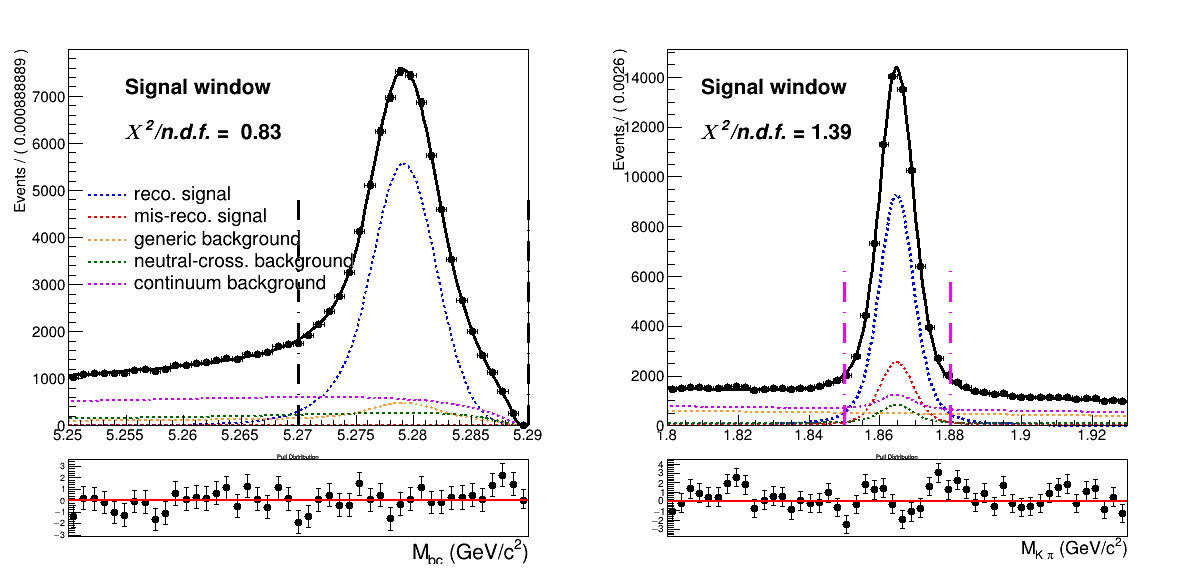
\includegraphics[width=0.75\textwidth]{A2-Appendix/figs/stream0Signal_window_chargedControlD0_Total_2DFit.png}}
\caption{Signal region ( $1.85 < M(\pi K) < 1.88$ GeV/c$^2$ and $5.27 < M_{bc} < 5.29$ GeV/c$^2$) projections of the two dimensional fit on stream0 (\cref{fig:stream0_chargedControlD0_Total_2DFit}).}
\label{fig:stream0Signal_window_chargedControlD0_Total_2DFit}
\end{figure}
 

  \begin{figure}[H]
%\centering
{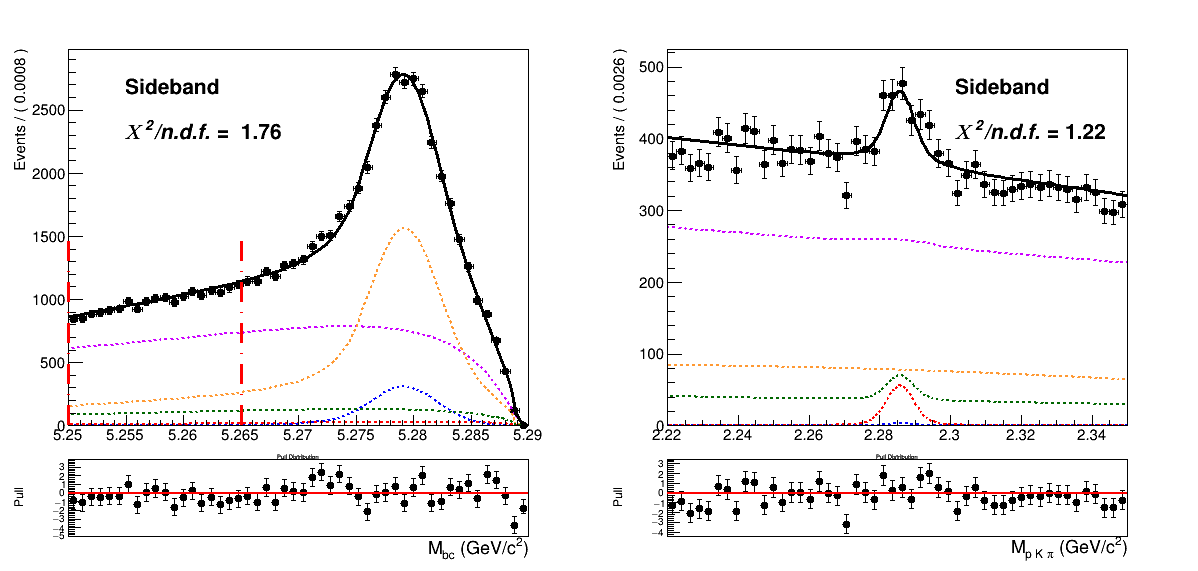
\includegraphics[width=0.75\textwidth]{A2-Appendix/figs/Mbc_Sideband_Total_2DFit_stream0_free_sigmas.png}}
\caption{Sideband region of $5.25 < M_{bc} < 5.265$ GeV/c$^2$ projection in $M(\pi K)$  of the two dimensional fit on stream 0.}
\label{fig:Mbc_Sideband_Total_2DFit_stream0}
\end{figure}
 
 \begin{figure}[H]
%\centering
{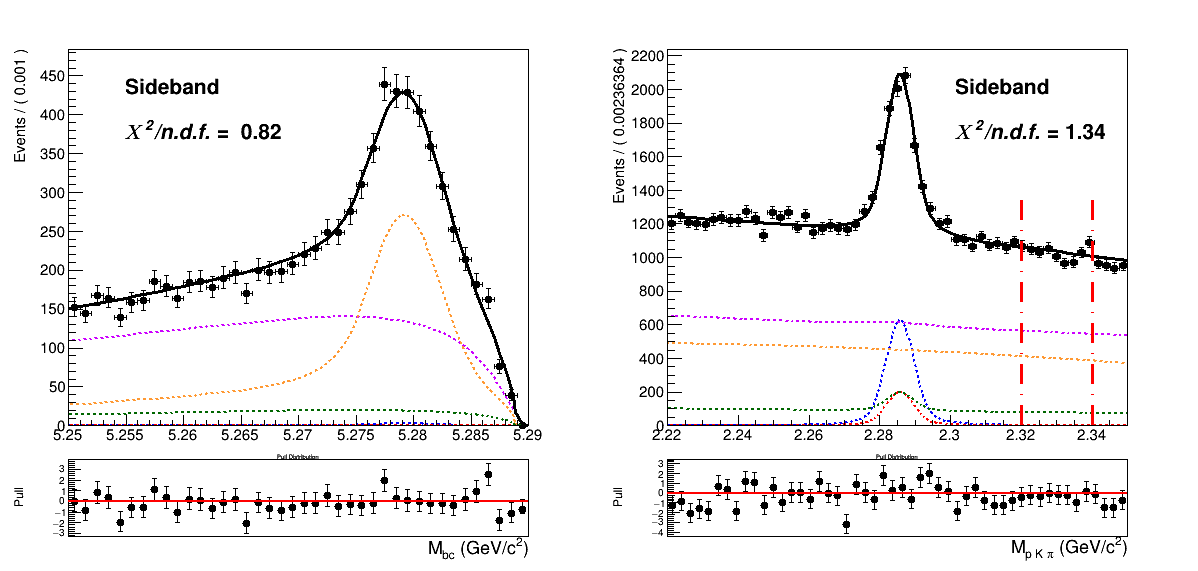
\includegraphics[width=0.75\textwidth]{A2-Appendix/figs/InvM_Sideband_Total_2DFit_stream0_free_sigmas.png}}
\caption{Sideband region of $1.8 < M(\pi K) < 1.84$ GeV/c$^2$ projection in $M_{bc}$ of the two dimensional fit on stream 0. }
\label{fig:InvM_Sideband_Total_2DFit_stream0}
\end{figure}

\crefrange{fig:Signal_window_chargedControlD0_Total_2DFit_onData_free_sigmaCB1_InvMsigma}{fig:InvMsideband_chargedControlD0_Total_2DFit_onData_free_sigmaCB1_InvMsigma} show the projections in $ M_{bc}$ and in the $D^0$ invariant mass of the two dimensional fit on data.

%\begin{figure}[h!]
%\centering
%{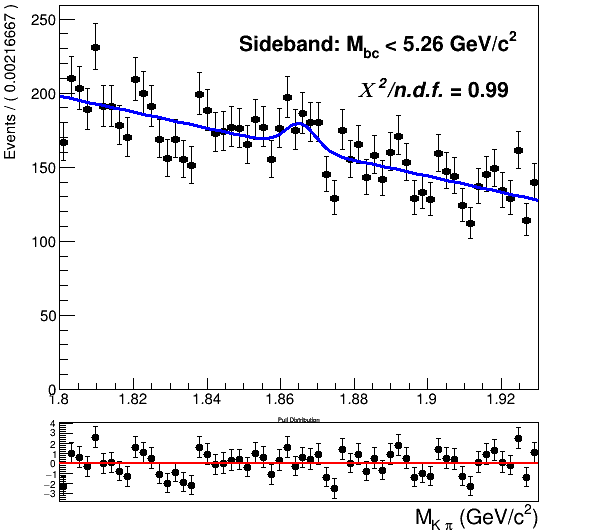
\includegraphics[width=0.50\textwidth]{A2-Appendix/figs/chargedControlD0_Generic_Mbc_SideBand_InvM.png}}
%\caption{projection of the sideband $M_{bc} < 5.26 GeV/c^2 $ region of the two dimensional fit shown in \cref{fig:chargedControlD0_Generic_2DFit} for generic background.}
%\label{fig:chargedControlD0_Generic_Mbc_5.26range_InvM}
%\end{figure}



 \begin{figure}[h!]
%\centering
{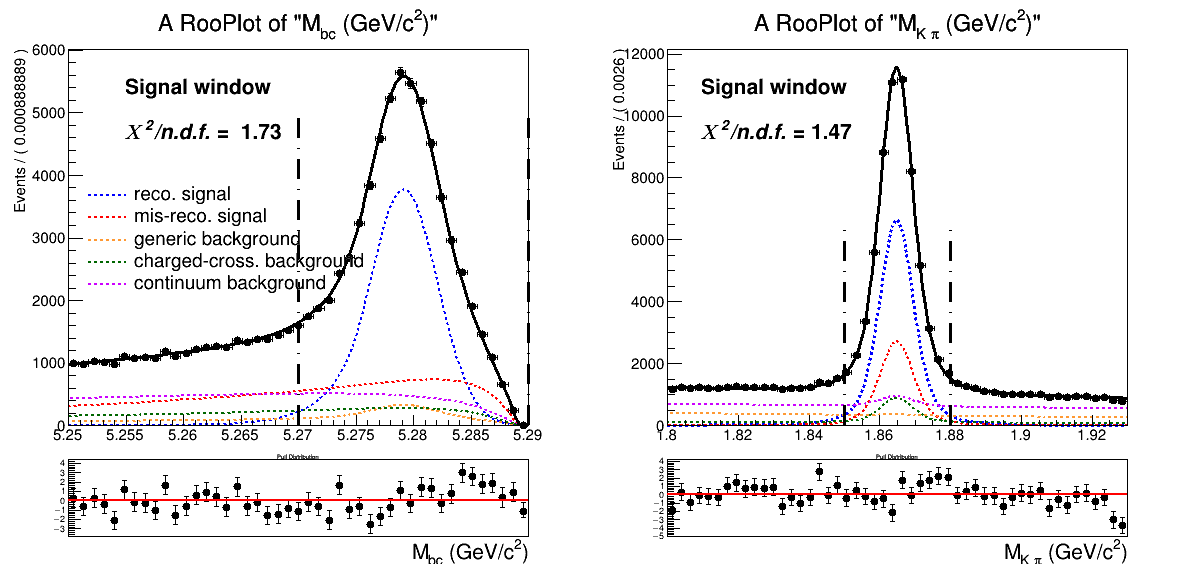
\includegraphics[width=0.75\textwidth]{A2-Appendix/figs/Signal_window_chargedControlD0_Total_2DFit_onData_free_sigmaCB1_InvMsigma.png}}
\caption{Signal region ( $1.85 < M(\pi K) < 1.88$ GeV/c$^2$ and $5.27 < M_{bc} < 5.29$ GeV/c$^2$) projections of the two dimensional fit on data described in \cref{chargedBtoD0_2Dfit_onData}}
\label{fig:Signal_window_chargedControlD0_Total_2DFit_onData_free_sigmaCB1_InvMsigma}
\end{figure}
 

  \begin{figure}[h!]
%\centering
{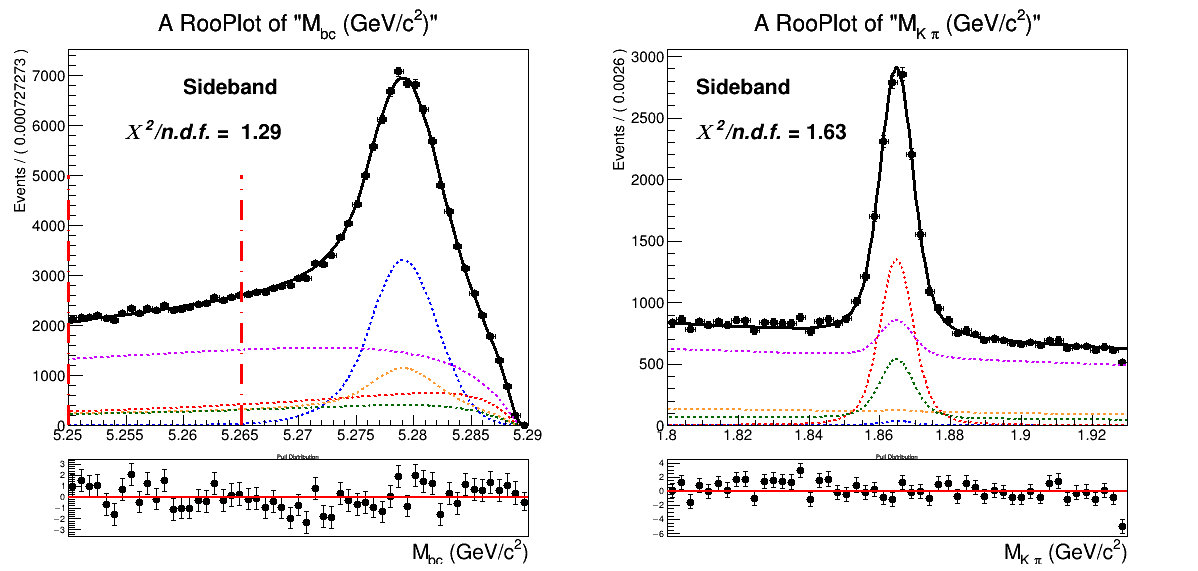
\includegraphics[width=0.75\textwidth]{A2-Appendix/figs/Mbc_sideband_chargedControlD0_Total_2DFit_onData_free_sigmaCB1_InvMsigma.png}}
\caption{Sideband region of $5.25 < M_{bc} < 5.265$ GeV/c$^2$ projection in $M(\pi K)$  of the two dimensional fit on data}
\label{fig:Mbc_sideband_chargedControlD0_Total_2DFit_onData_free_sigmaCB1_InvMsigma}
\end{figure}
 
 \begin{figure}[h!]
%\centering
{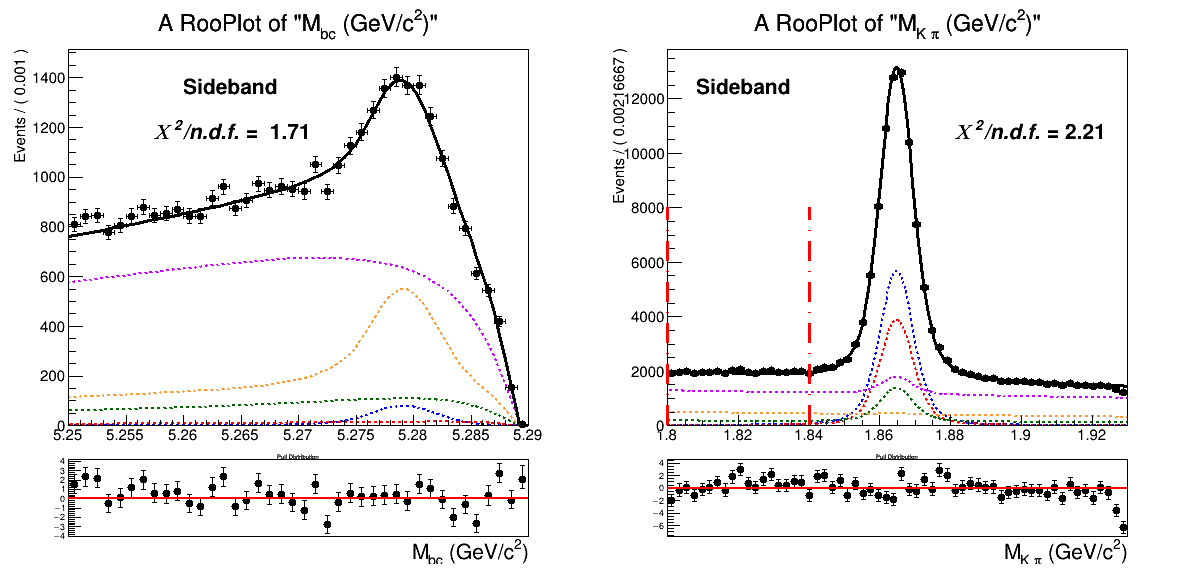
\includegraphics[width=0.75\textwidth]{A2-Appendix/figs/InvMsideband_chargedControlD0_Total_2DFit_onData_free_sigmaCB1_InvMsigma.png}}
\caption{Sideband region of $1.8 < M(\pi K) < 1.84$ GeV/c$^2$ projection in $M_{bc}$ of the two dimensional fit on data. }
\label{fig:InvMsideband_chargedControlD0_Total_2DFit_onData_free_sigmaCB1_InvMsigma}
\end{figure}
